\documentclass{beamer}
\usetheme{Boadilla}

\usepackage{algorithm2e}
\usepackage{amsmath}
\usepackage{amsfonts}
\usepackage{hyperref}

\usepackage{amsmath}
\DeclareMathOperator*{\argmax}{arg\,max}
\DeclareMathOperator*{\argmin}{arg\,min}


\title{AN INDUCTIVE BIAS FOR DISTANCES: NEURAL NETS
THAT RESPECT THE TRIANGLE INEQUALITY}
\author{Parviz Karimov}
\institute{MIPT, 2024}


\begin{document}

\begin{frame}
    \titlepage
\end{frame}


\begin{frame}
    \tableofcontents
\end{frame}


\section{Motivation \& Background}

\begin{frame}{Motivation}
    \begin{block}{}
    When defining distances, the triangle inequality has proven to be a useful constraint, both theoretically — to prove convergence and optimality guarantees — and empirically — as an inductive bias.
    \newline

    Deep metric learning architectures that
respect the triangle inequality rely, almost exclusively, on Euclidean distance in the
latent space. Though effective, this fails to model two broad classes of subadditive
distances, common in graphs and reinforcement learning: asymmetric metrics, and
metrics that cannot be embedded into Euclidean space.
    \end{block} 
\end{frame}

\begin{frame}{Example}
    \begin{figure}
        \centering
        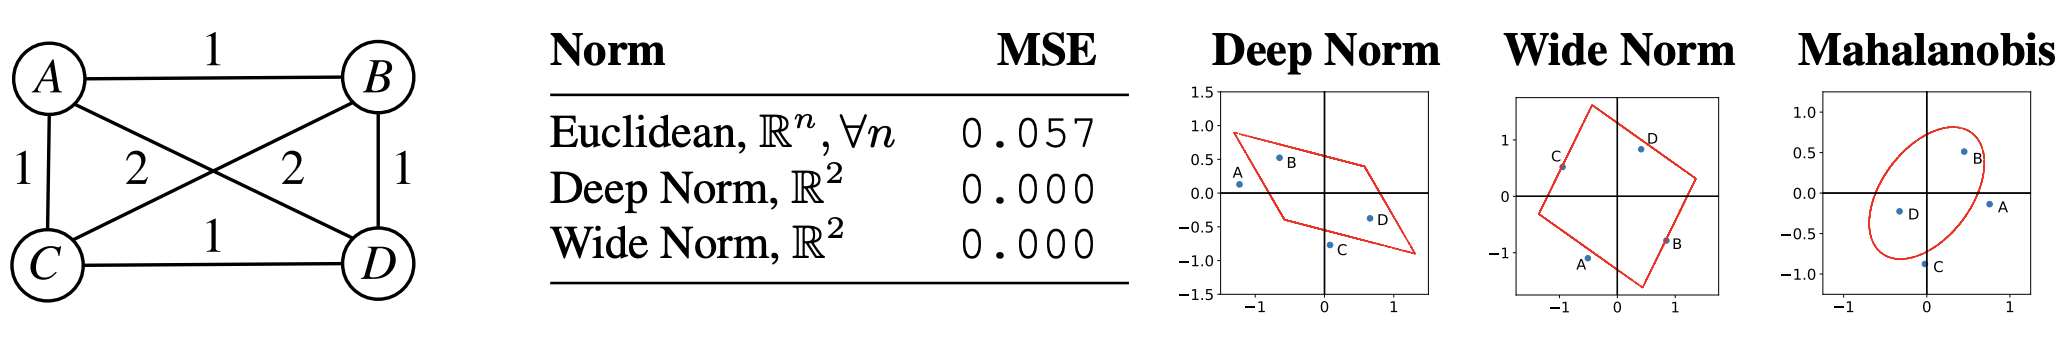
\includegraphics[width=\linewidth]{5.png}
        \caption{The nodes in the graph (left) cannot be embedded into any $\mathbb{R}^n$ so that edge distances are represented by the Euclidean metric: points $\phi(A)$ and $\phi(D)$ must lie at the midpoint of the segment
from $\phi(B)$ to $\phi(C)$—but then $\phi(A)$ and $\phi(D)$ coincide, which is incorrect. }
        \label{fig:enter-label}
    \end{figure}
\end{frame}


\begin{frame}{Background}
	\begin{block}{Metric}
        A \textbf{metric} is a function $d: \mathcal{X} \times \mathcal{X} \rightarrow \mathbb{R}^+$ satisfying $\forall x,y,z \in \mathcal{X}$
        \[
        \begin{align*}
        & \textbf{M1  } d(x, y) \geq 0 && \textbf{M3  } d(x, z) \leq d(x, y) + d(y, z) \\
        & \textbf{M2  } d(x, y) = 0 \iff x = y && \textbf{M4  } d(x, y) = d(y, x) \\
        \end{align*}
        \]
	\end{block}
    
    \begin{block}{Norm}
         A \textbf{norm} is a function $||\cdot||: \mathcal{X} \rightarrow \mathbb{R}^+$ satisfying $\forall x,y \in \mathcal{X}, \alpha \in \mathbb{R}^+$
         \[
        \begin{align*}
        & \textbf{N1  } ||x|| > 0 \text{ unless } x = 0 && \textbf{N3  } ||x + y|| \leq ||x|| + ||y|| \\
        & \textbf{N2  } \alpha ||x|| = ||\alpha x|| && \textbf{N4  } ||x|| = ||-x|| \\
        \end{align*}
         \]
    \end{block}

    \begin{block}{Convex function}
         Function $f : \mathcal{X} \rightarrow \mathbb{R}$ is called \textbf{convex} if
         \[
        \begin{align*}
        & \textbf{C1  } \forall x,y  \in \mathcal{X}, \alpha \in [0, 1] : f(\alpha x + (1 - \alpha)y) \leq \alpha f(x) + (1 - \alpha) f(y)
        \end{align*}
        \]
    \end{block}
\end{frame}

\begin{frame}{Background}
    \begin{block}{Auxilliary}
    A \textbf{quasi-metric} is \textbf{M1} and \textbf{M3}.

    An \textbf{assymetric norm} is \textbf{N1}-\textbf{N3}.

    An \textbf{(assymetric) semi-norm} is nonnegative, \textbf{N2} and \textbf{N3} (and \textbf{N4}).
    \end{block}

    \begin{block}{Prop. 0.1}
         Any assymetric semi-norm induces a quasi-metric. Any induces quasi-metric is translation-inveriant and positive homogeneous.
    \end{block}

    \begin{block}{Prop. 0.2}
         Any N2 and N3 function is convex — thus, all asymmetric semi-norms are convex.
    \end{block}
    
\end{frame}


\section{Deep Norm}
\begin{frame}{Deep Norm}
    \begin{block}{Proposition 1}
        All positive homogeneous convex functions are subadditive; i.e., $\textbf{C1} \wedge \textbf{N2} \implies \textbf{N3}$.
    \end{block}

    \begin{columns}
    \begin{column}{0.6\textwidth}
    \begin{figure}
        \centering
        \includegraphics[width=0.5\linewidth]{image.png}
        \caption{Deep norm architecture}
        \label{fig:enter-label}
    \end{figure}
    \end{column}

    \begin{column}{0.4\textwidth}
    
        \[
        \begin{align*}
            & ||x|| = h_k \\
            & h_i = g_i(W_i^+h_{i - 1} + U_ix) \\
            & h_0 = 0, W_1^+ = 0 \\
            & g_i \text{ preserves } \textbf{C1}, \textbf{N2} \\
            & g_k \text{ is non-negative} \\
            & W_i^+ \text{ is a non-negative matrix}
        \end{align*}
        \]
        
    \end{column}
    \end{columns}
\end{frame}

\begin{frame}{Deep Norm}

    \begin{block}{Proposition 2}
        If $||\cdot|$ is an assymetric semi-norm, then  $||x|| = ||x| + ||-x|$ is a semi-norm
    \end{block}

    \begin{block}{Proposition 3}
        if $||\cdot||_a$ is an assymetric semi-norm, $||\cdot||_b$ is a norm, $\lambda > 0$, then $||x||_{a + \lambda b} = ||x||_a + \lambda ||x||_b$ is an assymetric norm.
    \end{block}

    \begin{block}{Def. (MaxReLU)}
    \[
    \text{maxrelu}(x, y) = [\text{max}(x, y), \alpha \text{relu}(x) + \beta \text{relu}(y)], \quad \alpha,\beta \geq 0
    \]
    \end{block}
    
\end{frame}

\section{Wide Norm}
\begin{frame}{Wide Norm}
    \begin{block}{Def. (MaxMean)}
    \[
        \text{maxmean}(x_1, ..., x_n) = \alpha \text{max}(x_1, ..., x_n) + (1 - \alpha)\text{mean}(x_1, ..., x_n)
    \]
    \end{block}

    \begin{block}{Def. (Wide Norm)}
        A \textbf{Wide Norm} (or $k$-component mixture of Mahalanobis norms) is defined as 
        \[
        ||x|| = \text{maxmean}_i(||W_i x||_2), \text{ where } W_i \in \mathbb{R}^{m_i \times n}, m_i \leq n
        \]
    \end{block}
\end{frame}

\begin{frame}{Wide Norm}
    \begin{block}{Monotonic Norm (in the positive orthant)}
        \textbf{N5} $||\cdot||$ is \textbf{monotonic in the positive orthant} if $0 \leq x \leq y \implies ||x|| \leq ||y||$
    \end{block}

    \begin{block}{Proposition 4}
        if $||\cdot||$ is an \textbf{N5} (semi-)norm on $\mathbf{R}^{2n}$, then $||x|| = ||\text{relu}(x :: -x)||$ is an assymetric (semi-)norm on $\mathbb{R}^n$.
    \end{block}

    \begin{block}{Proposition 5}
        Mahalanobis norm with $W = DU$, with $D$ diagonal and $U$ non-negative, is \textbf{N5}.
    \end{block}
\end{frame}

\begin{frame}{Universal Approximation Theorem}
    \begin{block}{Theorem}
        The families $\mathcal{D}$ of Deep Norms (using MaxReLU)
and $\mathcal{W}$ of Wide Norms (using MaxMean) are dense in the family $\mathcal{N}$ of asymmetric semi-norms.
    \end{block}

\begin{figure}
    \centering
    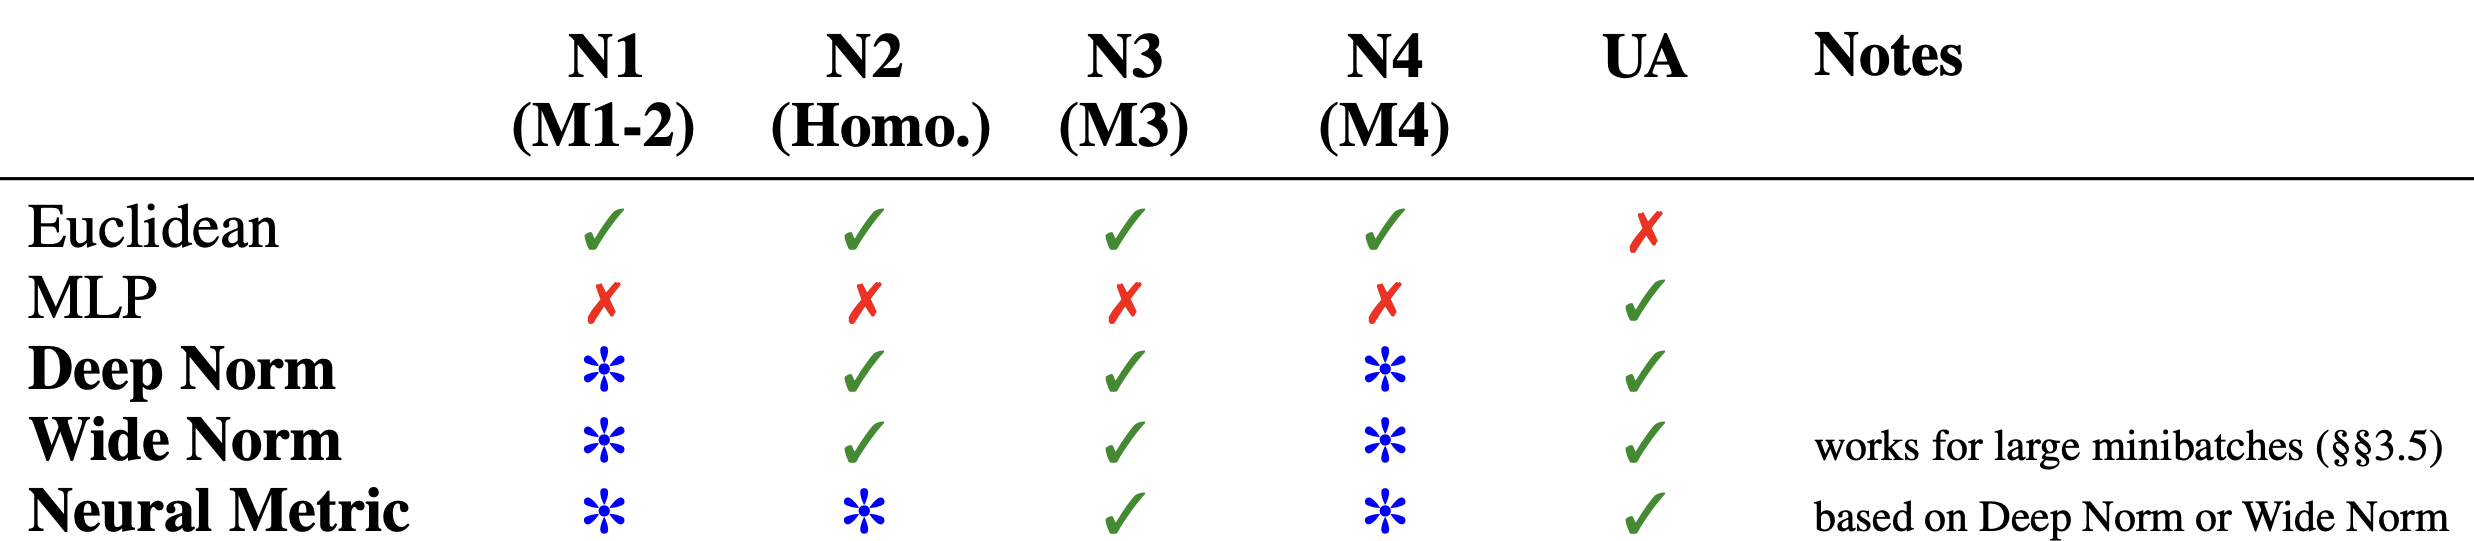
\includegraphics[width=\linewidth]{3.png}
    \caption{Norm (metric) properties of different architectures. As compared to Euclidean architectures,
ours are universal asymmetric semi-norm approximators (UA) and can use propositions to optionally
satisfy (*) \textbf{N1} and \textbf{N4}. Neural metrics relax the unnecessary homogeneity constraint on metrics.}
    \label{fig:enter-label}
\end{figure}
    
\end{frame}

\section{Application: Modelling Graph Distances}

\begin{frame}
    \begin{block}{}
    The task is of modeling shortest path lengths in a weighted graph $\mathcal{G} = (\mathcal{V}, \mathcal{E})$. So long as edge weights are
    positive and the graph is connected, shortest path lengths are discrete quasi-metrics ($n = |\mathcal{V}|$), and
    provide an ideal domain for a comparison to the standard Euclidean approach.
    \end{block}


\begin{figure}
    \centering
    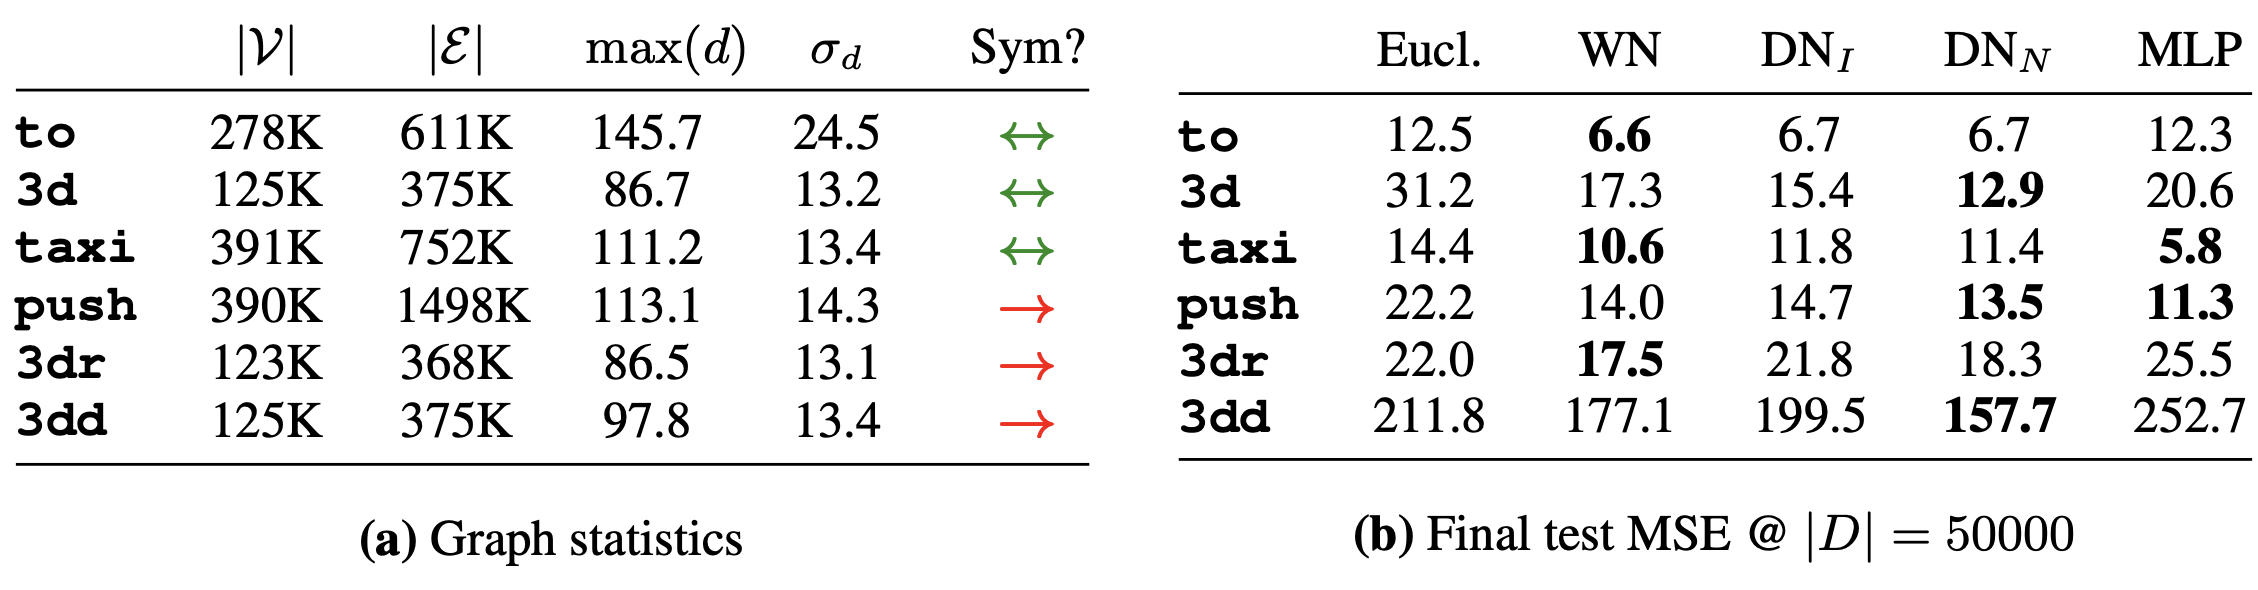
\includegraphics[width=\linewidth]{4.png}
    \caption{Graph experiments. (a) Statistics for different graphs. (b) Test MSE after 1000 epochs at
training size $|D|$ = 50000 (3 seeds). The best metric (and overall result if different) is bolded.}
    \label{fig:enter-label}
\end{figure}

\end{frame}

\section{Computational considerations}
\begin{frame}{Computational considerations}
    \begin{figure}
        \centering
        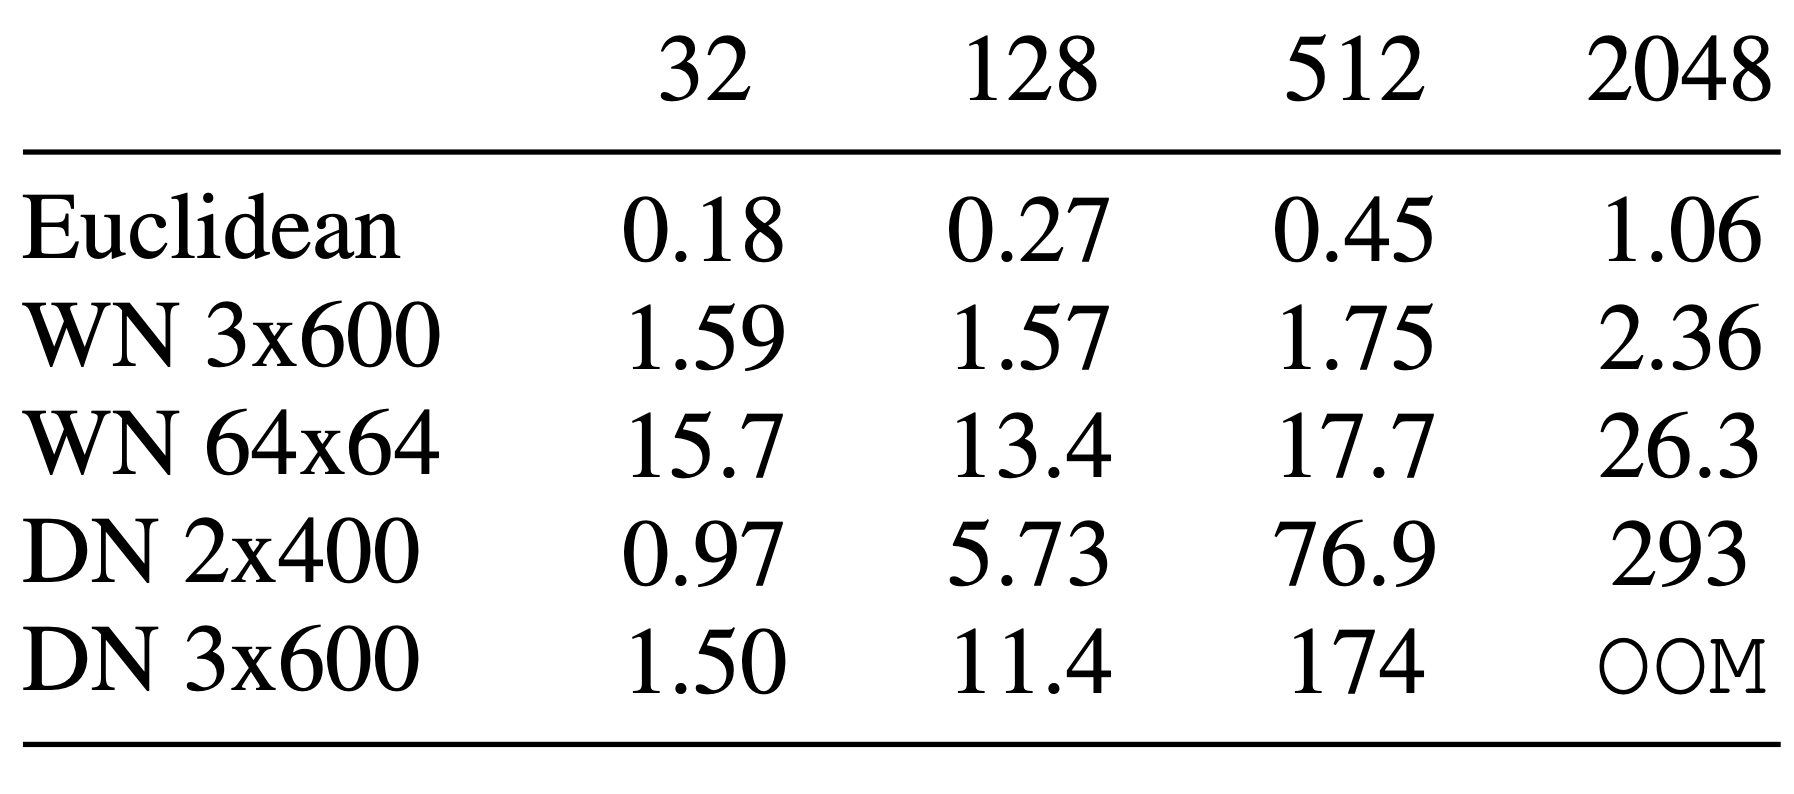
\includegraphics[width=0.5\linewidth]{6.png}
        \caption{Mean computation time (ms) for
    different mini-batch sizes (250 trials).}
        \label{fig:enter-label}
    \end{figure}
\end{frame}

\begin{frame}{Literature}
    \begin{enumerate}
        \item \textbf{Main article} \href{https://arxiv.org/pdf/2002.05825.pdf}
        {AN INDUCTIVE BIAS FOR DISTANCES: NEURAL NETS
THAT RESPECT THE TRIANGLE INEQUALITY}.
    \end{enumerate}
\end{frame}



\end{document}